%%=============================================================================
%% Proof-Of-Concept
%%=============================================================================


\chapter{Proof-Of-Concept}%
\label{ch:Proof-Of-Concept}


In dit hoofdstuk wordt omschreven op welke manier we onderzochte technologieën hebben toegepast op de probleemstelling van het bedrijf Lockit Rentals. De werking van eigen ontwikkelde toepassingen worden specifiek toegelicht op basis van gedocumenteerde informatie. Op vlak van de QR-codes is het doel om de huidige scan software te optimaliseren. Hierbij gaan er experimenten uitgevoerd worden om deze grondig te vergelijken. In het tweede deel zal de chatbot ontwikkeld worden aan de hand van het gekozen platvorm. Om aan te tonen dat nieuwe technieken een oplossing kunnen bieden, verwijs ik door naar de verwerkte resultaten \ref{ch:verwerkingresultaten}.

\section{Toepassingen QR-code scanners}%
\label{sec:toepassingenQR-coce scanners}

In dit onderzoek wordt dieper ingegaan op de QR-code camera’s. We nemen het script dat  op de locker units draait onder de loep. Het primair doel van deze aanpassing is het optimaliseren van de scanervaring voor toegangscodes. Door deze sneller en efficiënter te laten verlopen, gaan er zich minder problemen voordoen.

\subsection{Huidige toepassing QR-camera}
\label{sec:huidigeToepassingScanners}

In het hoofdstuk \ref{sec:WerkingUnits} wordt aangetoond welk script er effectief actief is op de locker units. Na grondig onderzoek van de gebruikte camera’s kunnen we concluderen dat deze geen specifieke toestellen zijn om QR-codes te scannen. De camera op zich heeft veel configuratie en rekenkracht nodig om de QR-code waar te nemen en te kunnen capteren in bruikbare data. 

Om deze experimenten uit te voeren, ga ik gebruik maken van een eigen opstelling die de huidige scanner inclusief de software hanteert te zien op figuur \ref{fig:vooraanzichtUSBCamera} en \ref{fig:achteraanzichtUSBCamera}. Uiteraard maak ik enkele aanpassingen aan de code om ervoor te zorgen dat deze geschikt is voor de vergelijking.  Het is belangrijk om op te merken dat deze wijzigingen geen invloed zullen hebben op de eindresultaten van de experimenten. Deze aangepaste code wordt weergegeven in listing \ref{lst:huidigeQR-codeData}.

\begin{figure}[h]
    \centering
    \begin{minipage}{0.45\textwidth}
        \centering
        \rotatebox{-90}{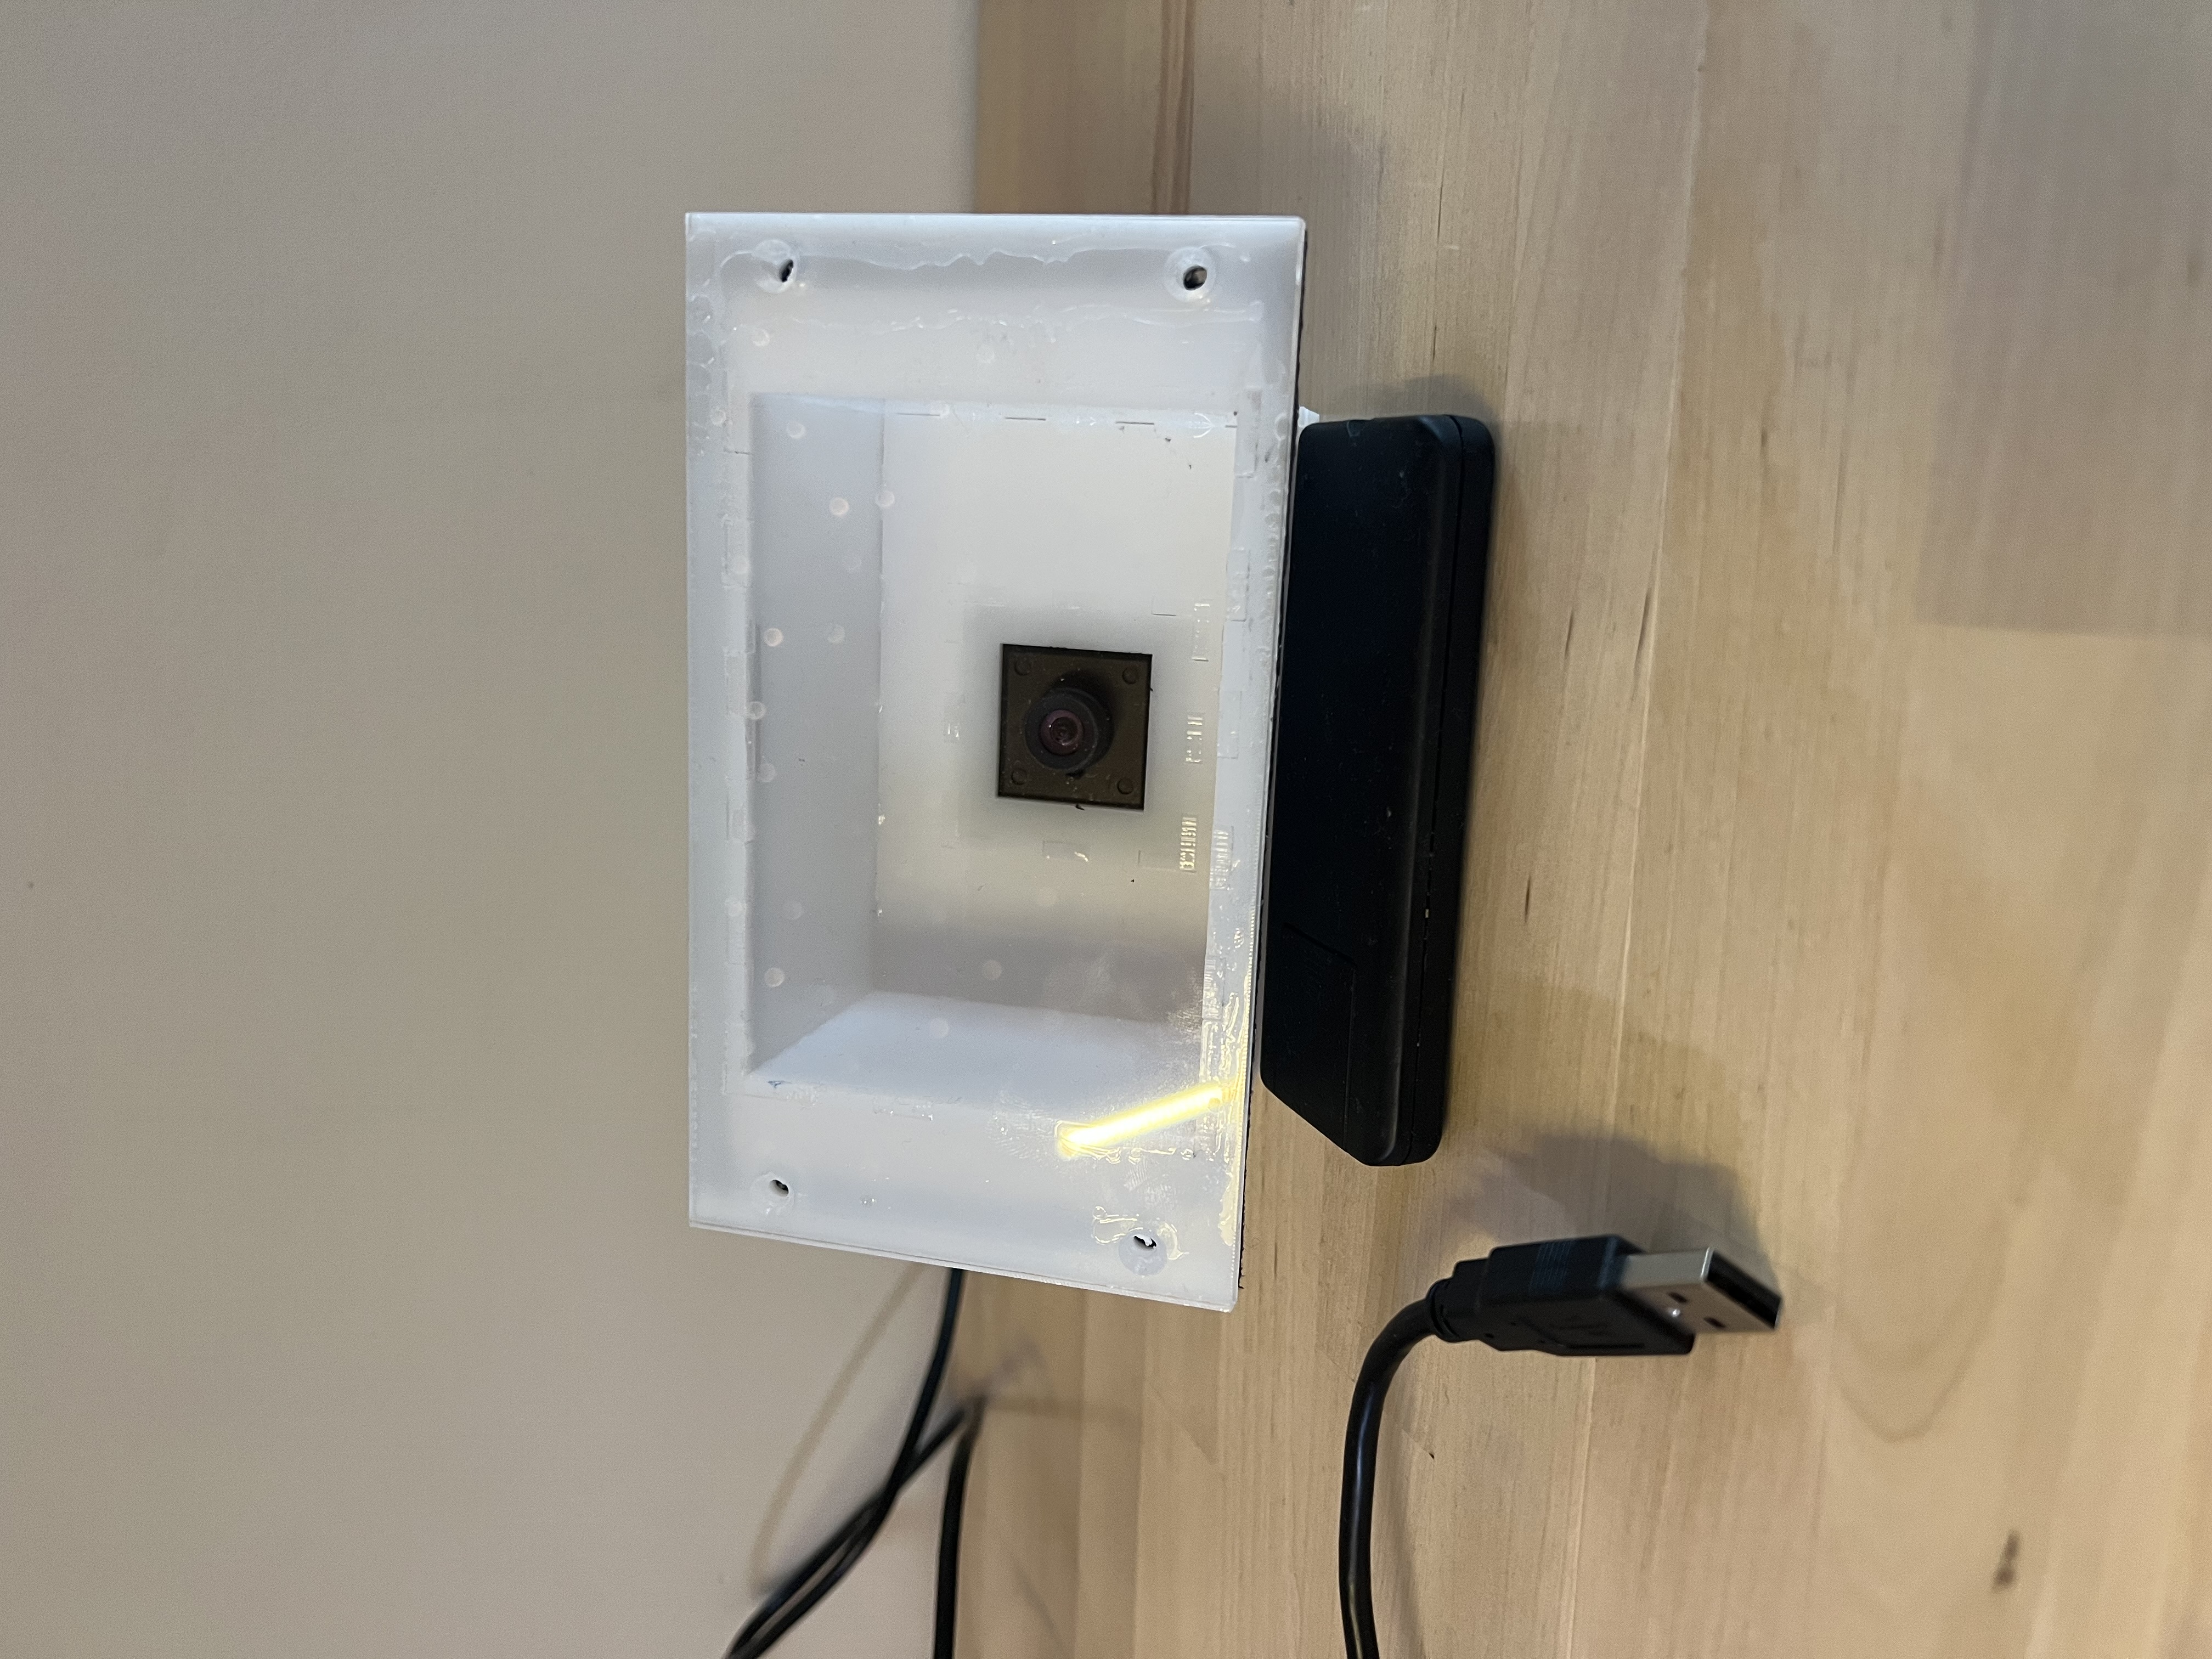
\includegraphics[width=\textwidth]{graphics/F22_USBCamera_front.jpeg}}
        \caption{Vooraanzicht USB QR-camera}
        \label{fig:vooraanzichtUSBCamera}
    \end{minipage}
    \hfill
    \begin{minipage}{0.45\textwidth}
        \centering
        \rotatebox{-90}{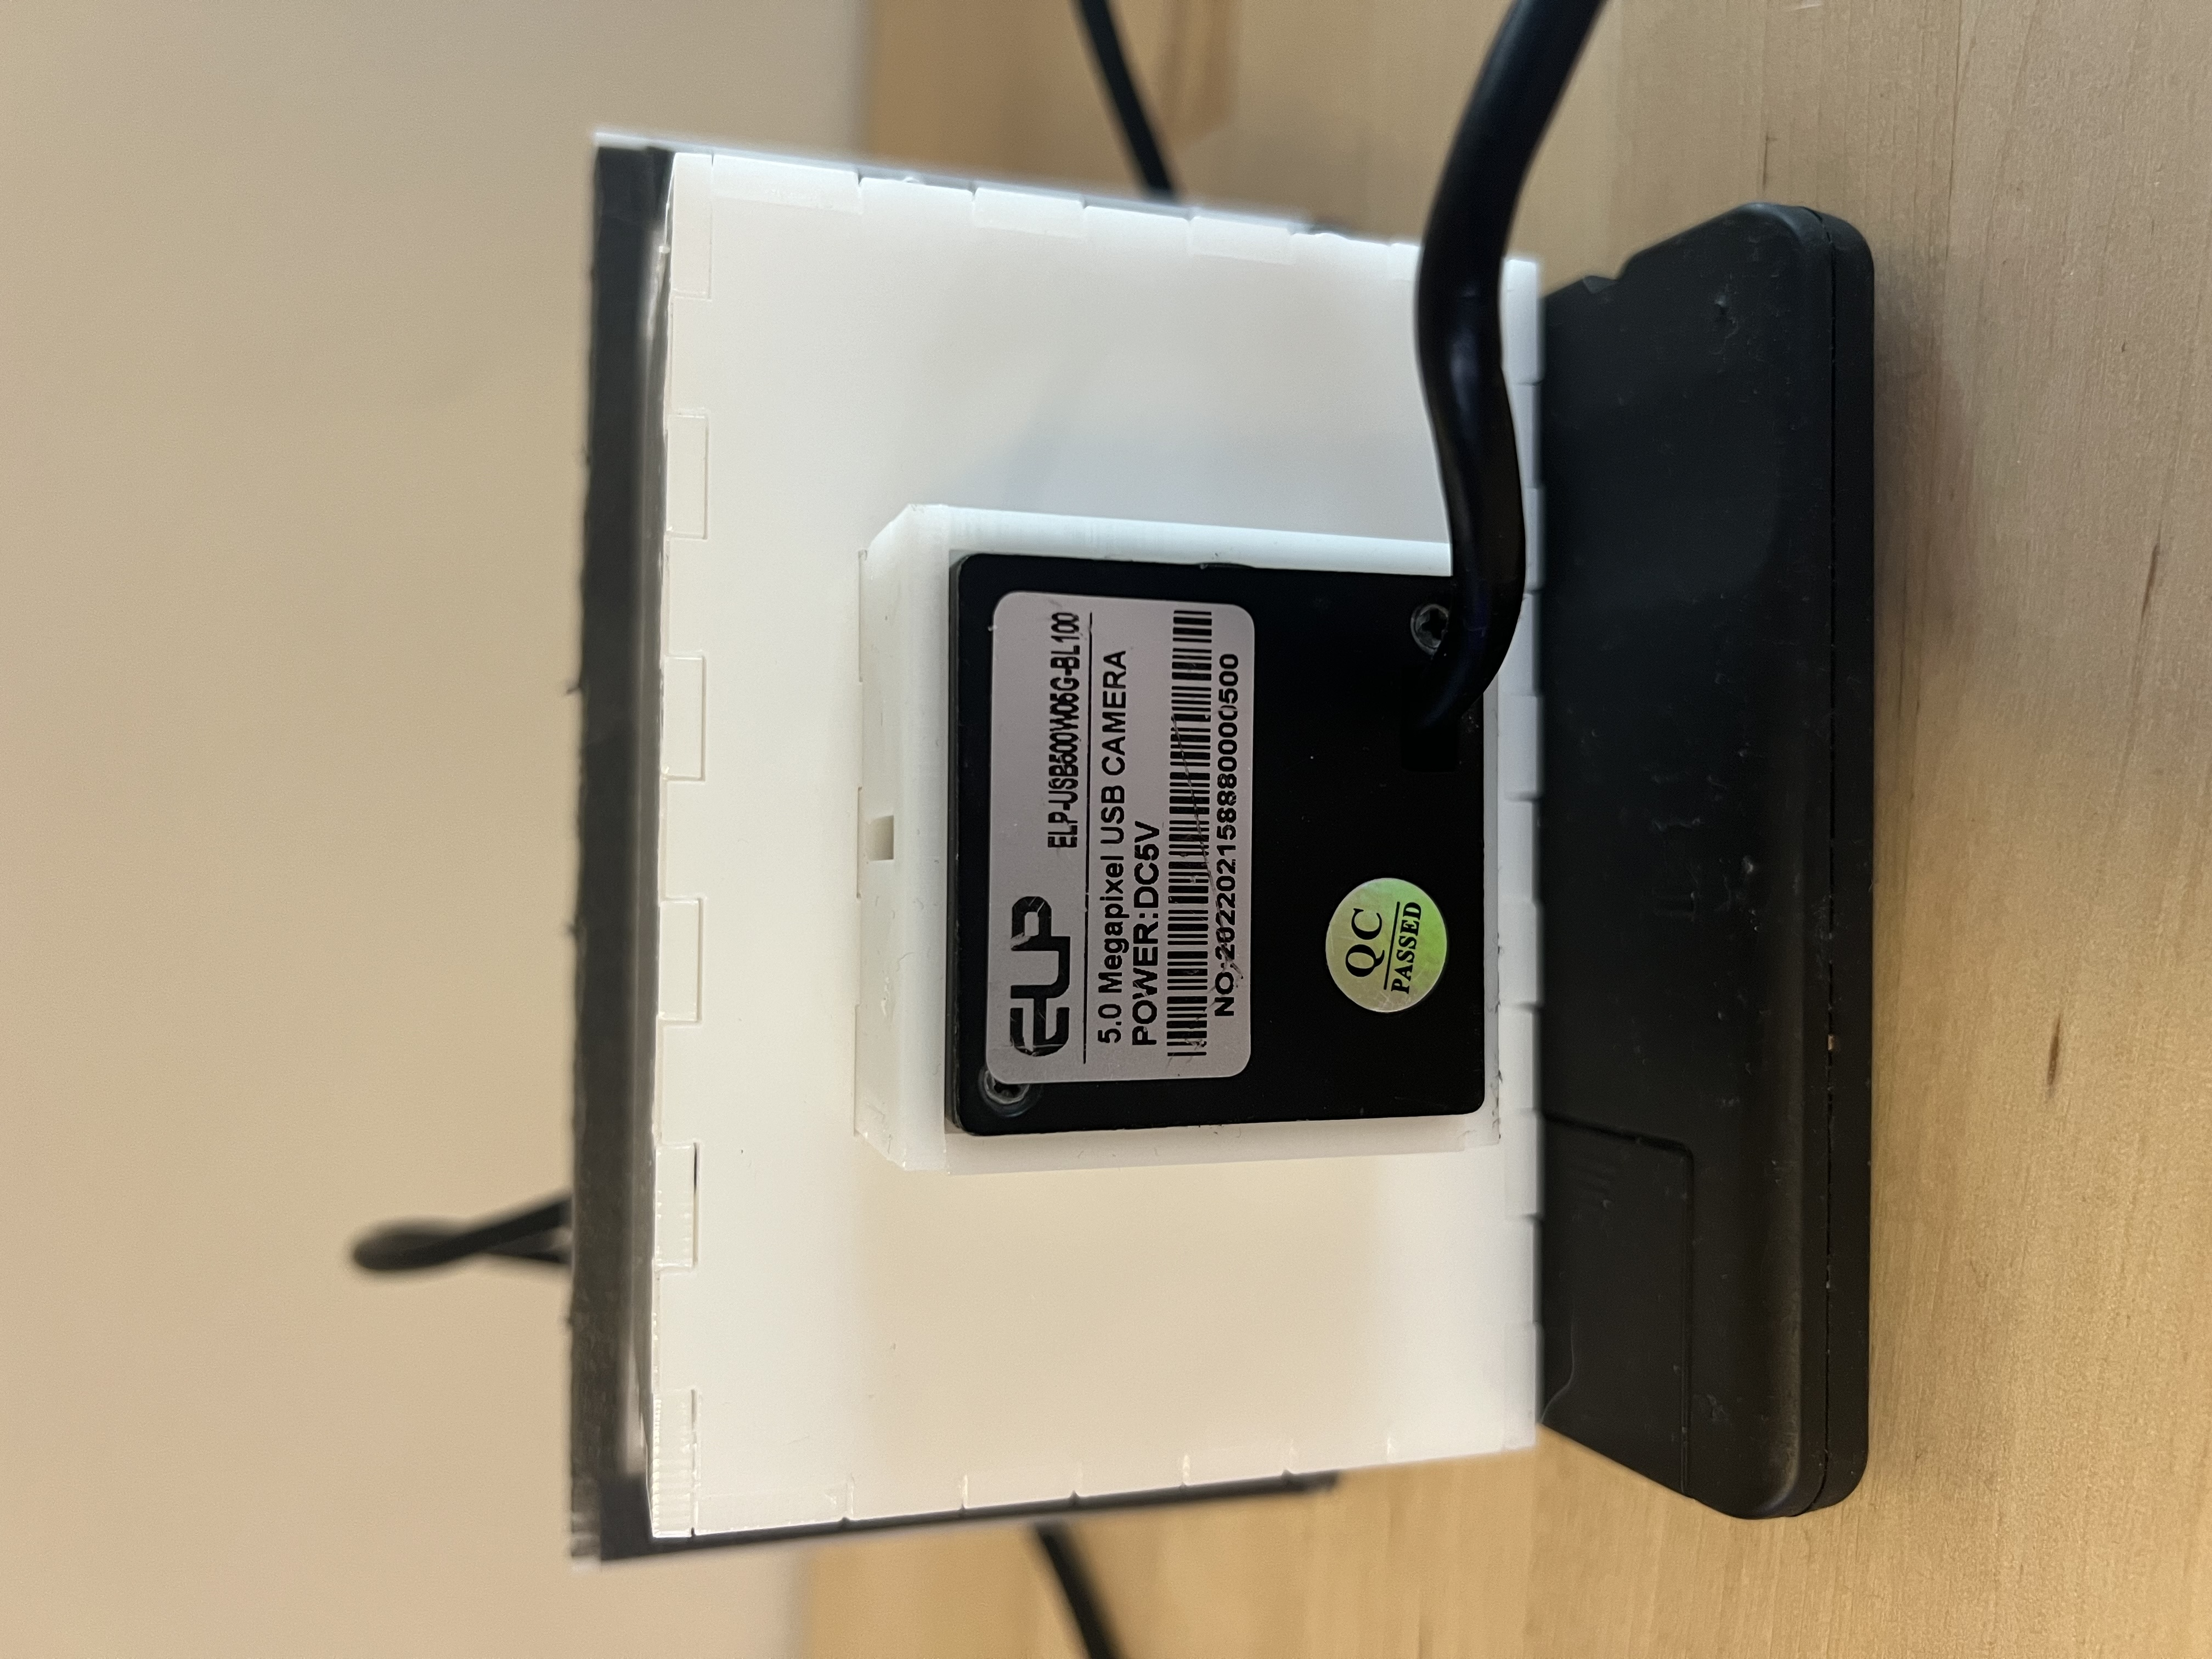
\includegraphics[width=\textwidth]{graphics/F23_USBCamera_back.jpeg}}
        \caption{Achteraanzicht USB QR-camera}
        \label{fig:achteraanzichtUSBCamera}
    \end{minipage}
    
\end{figure}



\begin{lstlisting}[language=Python, caption={Validatie van QR-code op tijd en bijpassende QR-unit.}, label=lst:huidigeQR-codeData, numbers=left]
    import cv2  # Importeer de cv2-bibliotheek voor het werken met beeldverwerking
    import time  # Importeer de time-bibliotheek om pauzes in de uitvoering van het programma te creëren
    import pyzbar.pyzbar as pyzbar  # Importeer de pyzbar-bibliotheek voor het decoderen van QR-codes
    from datetime import datetime  # Importeer de datetime-bibliotheek om tijdstempels te maken
    from openpyxl import Workbook  # Importeer de openpyxl-bibliotheek voor het werken met Excel-bestanden
    
    camera = cv2.VideoCapture(0)  # Gebruik de cv2-bibliotheek om toegang te krijgen tot de camera
    counter = 1  # Initialiseer een teller om bij te houden hoeveel QR-codes zijn gescand
    start_time = datetime.now()
    
    # Maak een nieuw werkboek / excel aan en selecteer het actieve werkblad
    workbook = Workbook()
    worksheet = workbook.active
    # Stel de kolomkoppen in voor het Excel-bestand
    worksheet['A1'] = 'Counter'
    worksheet['B1'] = 'Timestamp'
    worksheet['C1'] = 'Data'
    
    def decode_qr(image):  # Functie om QR-codes te decoderen
        try:
            gray = cv2.cvtColor(image, cv2.COLOR_BGR2GRAY)  # Zet het kleurenbeeld om in grijswaarden
            barcodes = pyzbar.decode(gray, symbols=[pyzbar.ZBarSymbol.QRCODE])  # Decodeer QR-codes
            if barcodes:
                timestamp = (datetime.now() - start_time).total_seconds()  # Bereken het tijdsverschil vanaf het begin
                timestamp_formatted = time.strftime('%H:%M:%S:%f', time.gmtime(timestamp))  # Maak de tijdstempel
                return (barcodes[0].data.decode(), timestamp_formatted)  # Return de gedecodeerde gegevens en tijdstempel
        except Exception as e:
            print(e)
        return None
    
    while counter <= 50:
    ret, frame = camera.read() # Lees de afbeelding van de camera
    
        if not ret:
            break
        qr_data = decode_qr(frame) # Decodeer QR-code in afbeelding
        if qr_data:
            timestamp = (datetime.now() - start_time).total_seconds() * 1000 # Formatteer de timestamp
            hours, remainder = divmod(int(timestamp), 3600000)
            minutes, remainder = divmod(remainder, 60000)
            seconds, milliseconds = divmod(remainder, 1000)
            timestamp_formatted = f"{hours:02}:{minutes:02}:{seconds:02}:{milliseconds:03}"
            # Print de QR-code informatie en voeg het toe aan de Excel-sheet
            print(f'{counter} | Timestamp: {timestamp_formatted} | Data: {qr_data[0]}')
            # Normaal doen we hier het POST request naar de server zie originele code
            row = (counter, timestamp_formatted, qr_data[0])
            worksheet.append(row)
            counter += 1
        time.sleep(3) # Wacht 3 seconden tussen elke frame
    
    
    end_time = datetime.now()
    
    # Sla het Excel bestand op
    workbook.save('qr_codes_records_camera_normaal_gsm_120lux.xlsx')
    
    print(f"Counter reached {counter - 1}. Exiting program. Final time of scanning: {end_time - start_time}")
    camera.release() # Beëindig het gebruik van de camera   
    
\end{lstlisting}
